\begin{figure}[!t]
\centering
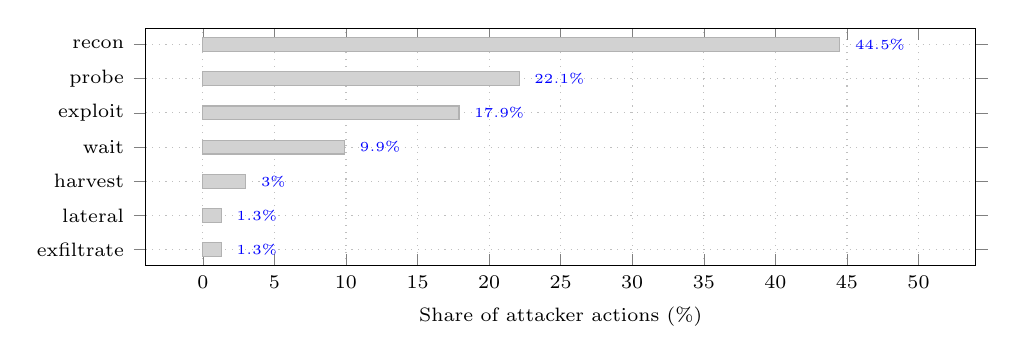
\begin{tikzpicture}
\begin{axis}[
  xbar,
  bar width=5pt,
  width=\columnwidth,
  height=4.6cm,
  xmin=0, xmax=50,
  xlabel={Share of attacker actions (\%)},
  symbolic y coords={exfiltrate, lateral, harvest, wait, exploit, probe, recon},
  ytick=data,
  yticklabel style={font=\scriptsize},
  xticklabel style={font=\scriptsize},
  label style={font=\scriptsize},
  nodes near coords={\pgfmathprintnumber[precision=1]{\pgfplotspointmeta}\%},
  nodes near coords align={horizontal},
  every node near coord/.append style={font=\tiny, xshift=2pt},
  grid=major,
  major grid style={dotted,gray!50},
  enlargelimits=0.08,
]
\addplot+[fill=gray!35, draw=gray!60] coordinates {
(1.3,exfiltrate) (1.3,lateral) (3.0,harvest) (9.9,wait)
(17.9,exploit) (22.1,probe) (44.5,recon)
};
\end{axis}
\end{tikzpicture}
\caption{Attacker action mix on hybrid B4 episodic run (seed~540,
$30$ episodes). Counts aggregate all attacker tool invocations; the
kill chain appears as a long tail of $\mathtt{recon}$ and
$\mathtt{probe\_service}$ before occasional $\mathtt{exfiltrate}$.}
\label{fig:action-mix}
\end{figure}
